\documentclass[12pt]{article}
\usepackage[spanish]{babel}
\usepackage{lipsum}
% *** GRAPHICS RELATED PACKAGES ***
\usepackage{graphicx}       % Loading images
\graphicspath{{./figuras/}} % Figures relative directory
\usepackage{subcaption} 	% For subfigures
\usepackage{wrapfig}		% Text wrapped around figure
\usepackage{overpic}		% To add text over figures

\usepackage{rotating}

\usepackage[colorlinks]{hyperref}

\begin{document}

\section{Primer sección}

Esto es un texto de relleno sin sentido. Tengo la Figura \ref{fig:leon}.


\includegraphics[width=0.3\linewidth]{figuras/leon}

\begin{figure}[h]
	\centering
	
\includegraphics[width=0.4\linewidth]{figuras/leon}
	\caption{Esto es una leyenda.}
	\label{fig:leon}
\end{figure}

\begin{figure}[h]
	\centering
	\begin{subfigure}{.45\textwidth}
		\centering
		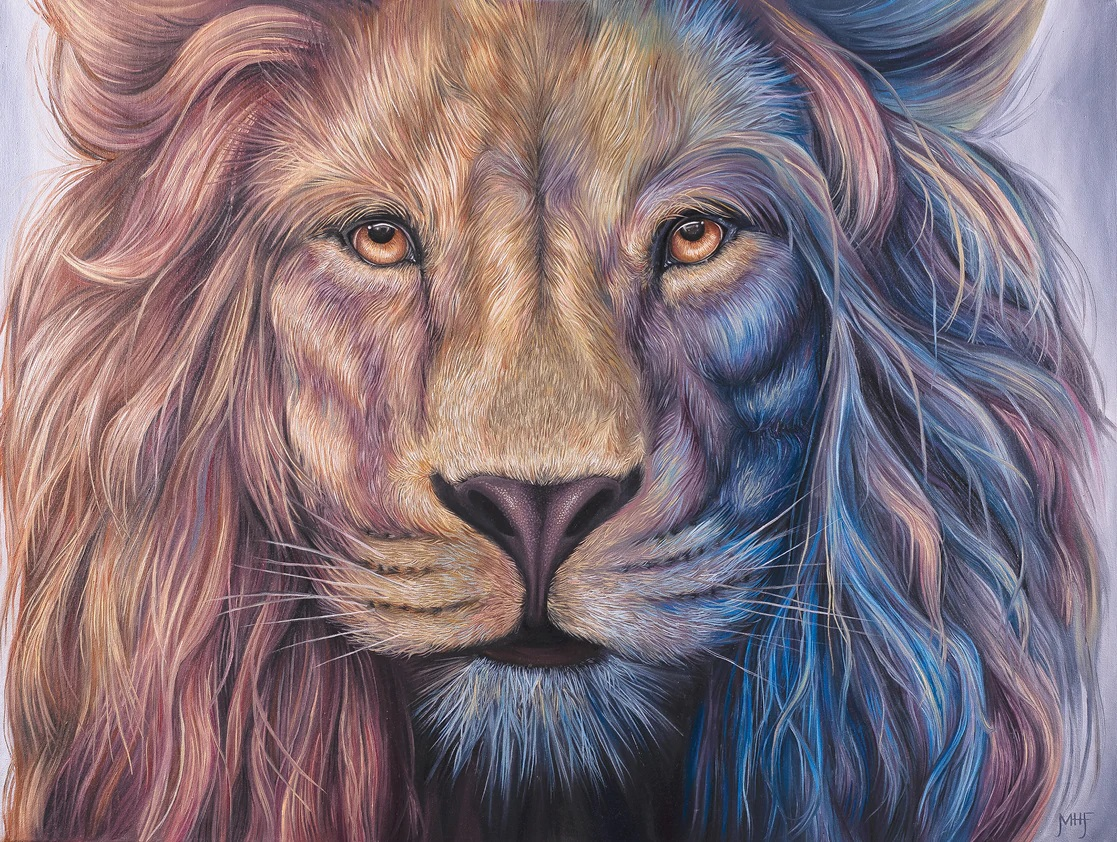
\includegraphics[width=1\textwidth]{leon1}%
		\caption{Un león.}
		\label{fig:leon1}
	\end{subfigure} 
	\hfil
	\begin{subfigure}{.45\textwidth}
		\centering
		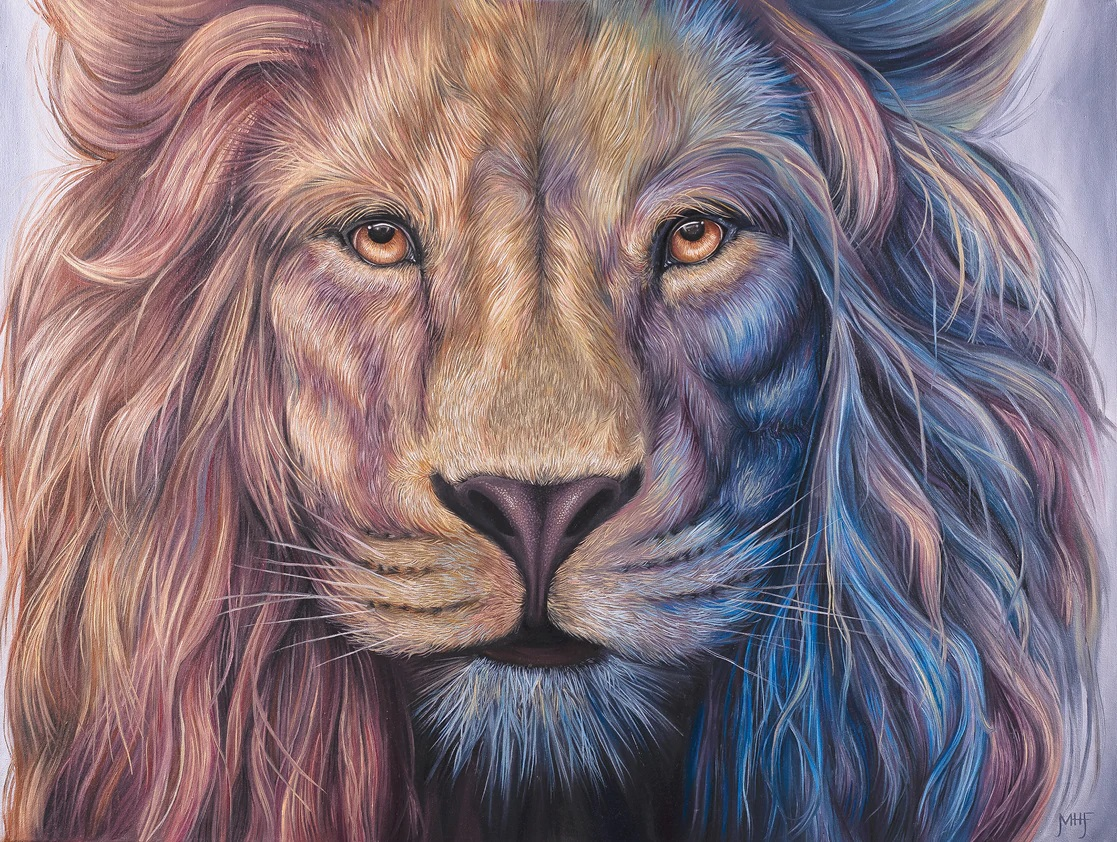
\includegraphics[width=1\textwidth]{leon1}%
		\caption{Otro león.}
		\label{fig:leon2}
	\end{subfigure}
	\caption{Este es un caso en donde se pueden poner dos imágenes juntas, se tiene la Figura \ref{fig:leon1} y por otro lado se tiene la Figura \ref{fig:leon2}.}
	\label{fig:leones}
\end{figure}

\begin{figure}[h]
	\centering
	\begin{subfigure}{.45\textwidth}
		\centering
		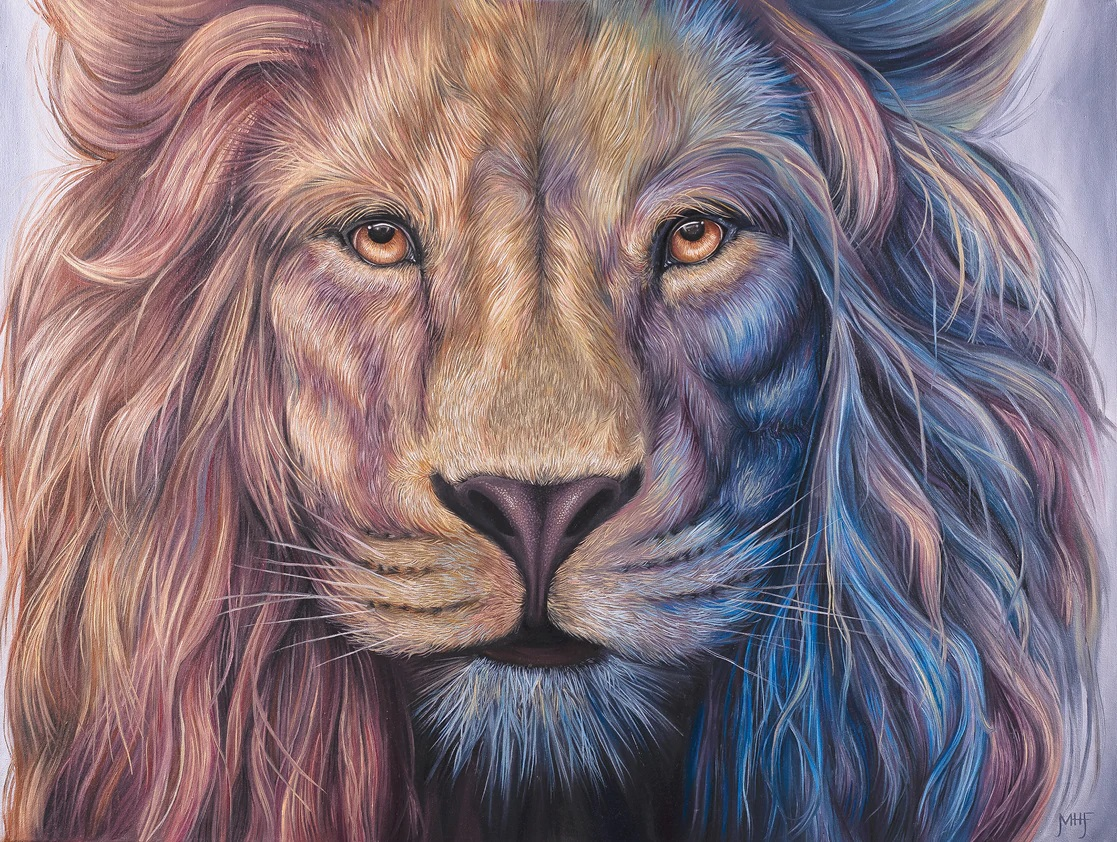
\includegraphics[width=1\textwidth]{leon1}%
		\caption{Un león.}
	\end{subfigure} 
	\hfil
	\begin{subfigure}{.45\textwidth}
		\centering
		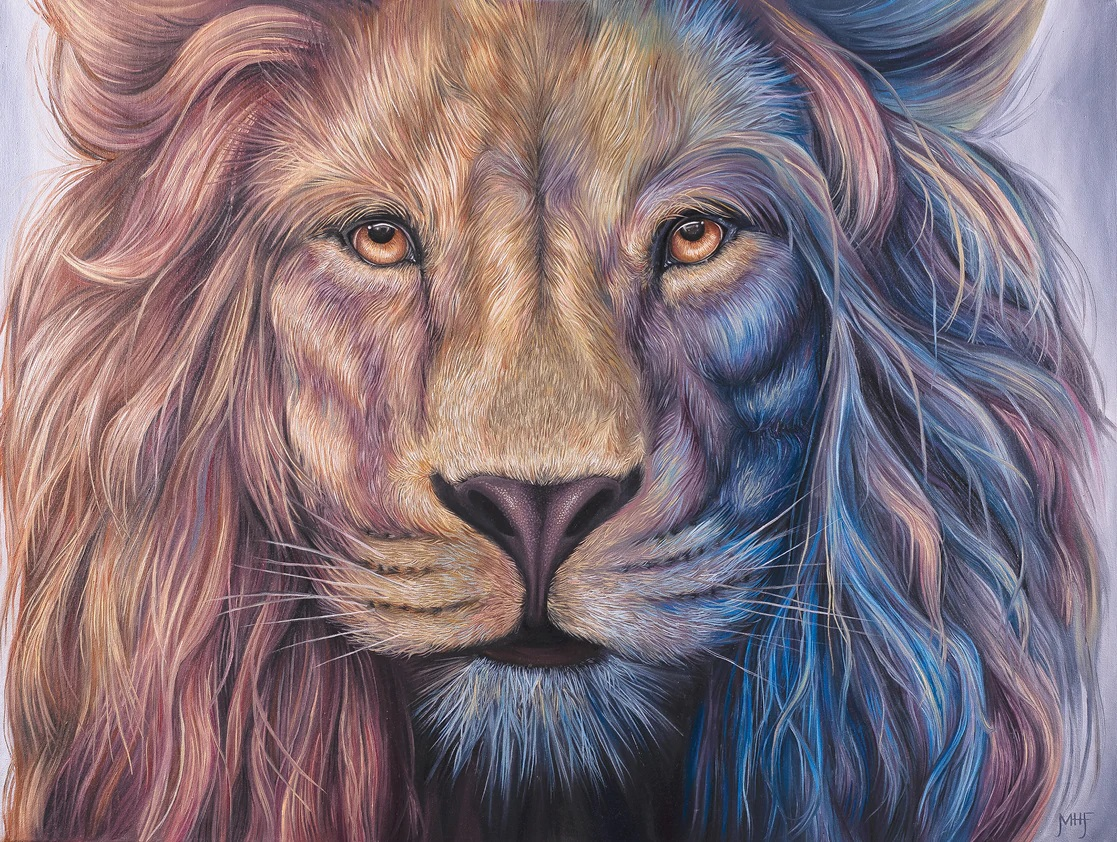
\includegraphics[width=1\textwidth]{leon1}%
		\caption{Otro león.}
	\end{subfigure} \\
	\begin{subfigure}{.45\textwidth}
		\centering
		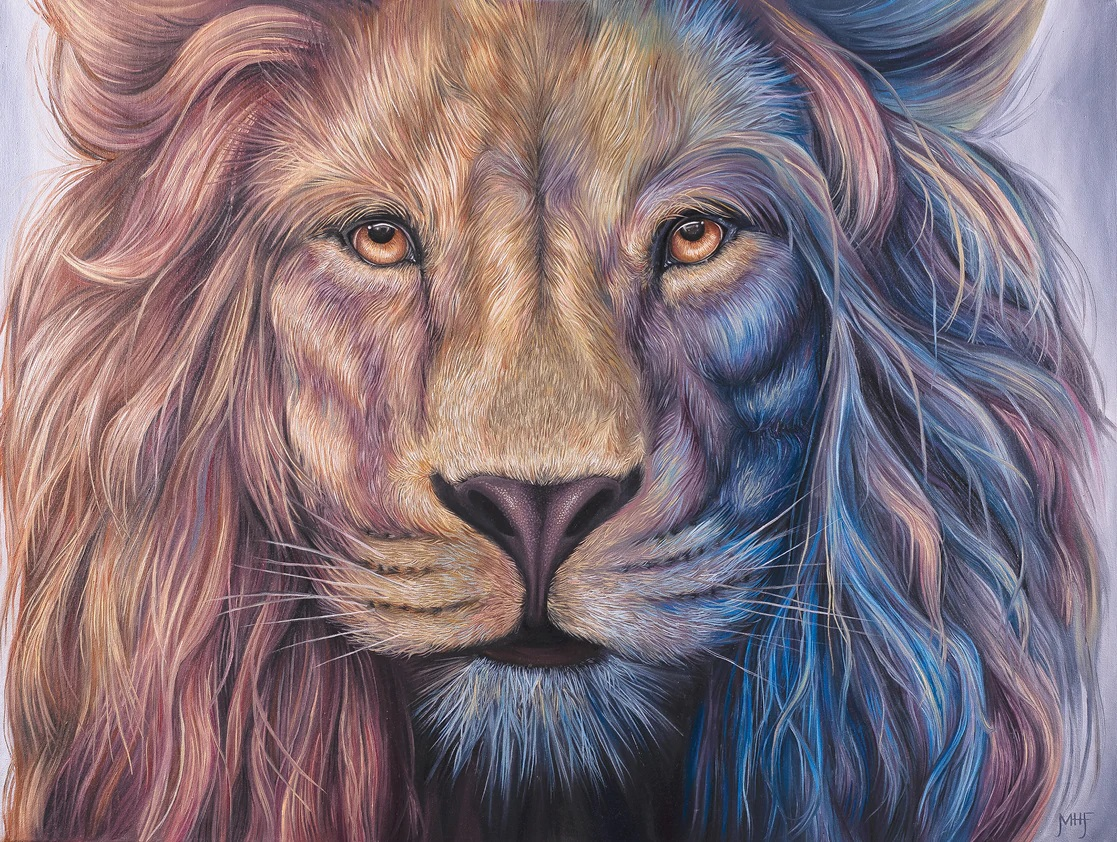
\includegraphics[width=1\textwidth]{leon1}%
		\caption{Un león.}
	\end{subfigure} 
	\hfil
	\begin{subfigure}{.45\textwidth}
		\centering
		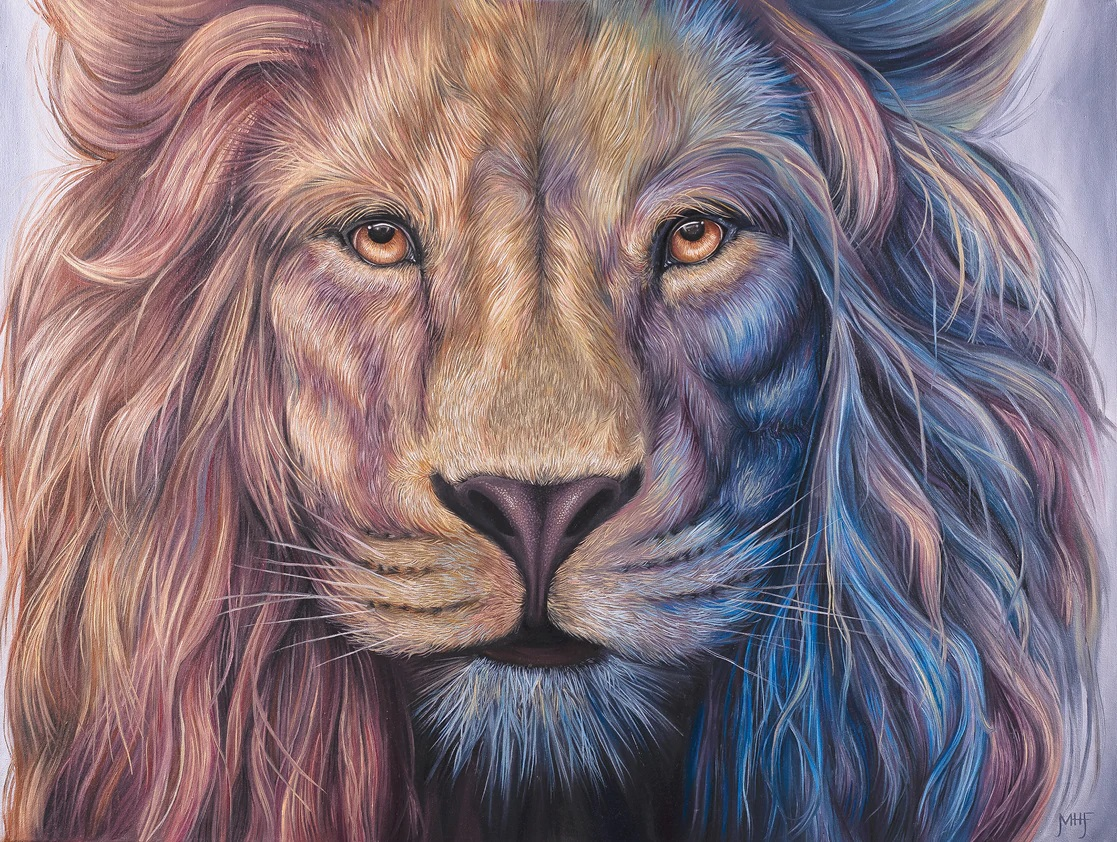
\includegraphics[width=1\textwidth]{leon1}%
		\caption{Otro león.}
	\end{subfigure}
	\caption{Este es un caso en donde se pueden poner dos imágenes juntas, se tiene la Figura \ref{fig:leon1} y por otro lado se tiene la Figura \ref{fig:leon2}.}
	\label{fig:leones2}
\end{figure}
\newpage
\section{Texto al lado de la figura}

\begin{wrapfigure}[10]{l}{0.4\linewidth}
	\vspace{-17pt}
	
\includegraphics[width=1\linewidth]{leon2}
\end{wrapfigure}
\lipsum[1]

\section{Figura con texto arriba}

\begin{figure}[h]
	\centering
	\begin{overpic}[width=0.7\textwidth,tics=5]{leon3} % Write ",grid" after tics to activate it. "tics" defines the grid spacing.
		\put (10,77) { Nariz }
		\put (3,28) { Barbilla }
		\put (79,88) { Melena }
	\end{overpic}
	\caption{Partes de un león.}
	\label{fig:overpic}
\end{figure}
\newpage
\begin{sidewaysfigure}
	\centering
	
\includegraphics[width=1\linewidth]{figuras/leon4}
	\caption{Esto es una leyenda.}
	\label{fig:leon5}
\end{sidewaysfigure}

\end{document}
